\chapter{\textit{Machine Learning} e Análise de Sentimentos}

\section{Contextualização}
\label{sec:methods}

Os problemas tratados por \textit{Machine Learning} classificam-se de forma
geral em três tipos:

\begin{itemize}
	\item Aprendizado supervisionado: nesse caso tem-se os elementos de entrada e
	para cada um desses elementos, tem-se associado um rótulo. Nesse caso o modelo
	deve ser treinado com base nos elementos dados para que se possa prever o rótulo %	não consegui pensar numa tradução boa pra label%
	de uma nova entrada;
	\item Aprendizado não-supervisionado: nesse caso tem-se apenas os elementos de entrada. 
	O objetivo deste tipo de problema é tentar modelar uma distribuição ou estrutura comum
	entre os dados para que se possa entendê-los melhor;
	\item Aprendizado semi-supervisionado: nesse último caso alguns elementos possuem um rótulo
	associado. Problemas desse tipo aplicam técnicas tanto de aprendizado supervisionado como
	de não-supervisionado.
\end{itemize}

\section{O problema da classificação}

Neste trabalho será tratado um problema de aprendizado supervisionado que é o da classificação.
No problema de classificação, tem-se $K$ classes $\{1, \ldots, K\}$ com $K \ge 2$ e o objetivo
é treinar um modelo que, para uma dada entrada $x \in \mathbb{R}^m$, determine qual classe ela
pertence.

Um exemplo de problema classificação é o caso do \textit{iris dataset} onde se classifica uma
flor iris entre três tipos \textit{Iris setosa}, \textit{Iris virginica} e \textit{Iris versicolor}
baseado nos tamanhos das pétalas e sépalas.

Para a etapa de treinamento, utiliza-se um conjunto $X = (x_1, x_2, \ldots, x_n)$ e para cada
$x_i \in \mathbb{R}^m$ está associado um $t_i \in \{1, \ldots, K\}$. Será usado $n$ para o
tamanho do conjunto de entrada e $m$ para o tamanho de cada vetor.
Os modelos de classificação que serão discutidos neste trabalho realizam a etapa de treinamento
resolvendo um problema de otimização que tem como fim direta ou indiretamente diminuir o erro
associado a classificação de um elemento, além disso é necessário que o modelo final tenha
boa generalização, isto é, apresente baixo erro para a classificação de novas amostras além das
presentes no conjunto de entrada.

Qual função objetivo a ser otimizada e como fazer isso varia para cada método uma vez que
um método não necessariamente se aplica a demais.

Como será discutido mais a frente no capítulo, cada modelo possui diferentes abordagens para o
caso binário e o caso multiclasses, porém os fundamentos são os mesmos portanto será explicado
tanto para a regressão logística quanto para o SVM o caso binário e depois irá estender para
o problema a ser resolvido neste trabalho.


\section{Logistic Regression}
\label{sec:logreg} 

Na regressão logística o modelo de classificação é probabilístico o que significa
que, a partir de um discriminante linear atribui-se a probabilidade do
elemento $x$ percenter à classe $C^1$, denotada por $P(C^1 | x)$. O discriminante
linear é dado pela equação: 
\begin{center}
	\begin{equation}
		\label{eq:lin_discriminant}
		f(x) = w^Tx + w_0,
	\end{equation}
\end{center}
o vetor $\tilde{w} = (w, w_0)$
é chamado de vetor de pesos e o termo $w_0$ é chamado de viés.
Para efeitos de contas
será usado $w$ para se referir ao vetor $\tilde{w}$ e o vetor x será dado por $x = (x_{original}, 1)$.

Utilizando \ref{eq:lin_discriminant} obtém-se a probabilidade $P(C^1 | x)$ utilizando a função sigmóide
sobre $f(x)$ que é dado por:

\begin{center}
	\begin{equation}
		\label{eq:sigmoid_y}
		P(C^1 | x) = y(x) = \sigma(f(x)) = \frac{1}{1 + e^{-f(x)}}
	\end{equation}
\end{center}
e consequentemente $P(C^2 | x) = 1 - P(C^1 | x)$.
A classe ao qual um elemento $x$ pertence é aquela que possui maior probabilidade. Utiliza-se
a sigmoide, pois a função possui a propriedade de mapear o conjunto dos números reais no intervalo
$[0, 1]$.

No caso da classificação binária, o rótulo de um elemento $t_i$ corresponde a 1 se o elemento $x_i$
pertence à classe $C^1$ e 0 se pertence a $C^2$.

O objetivo do processo de treinamento da regressão logística é obter um vetor $w$ que minimize
o erro da classificação. Para obter-se a função de erro, primeiro calcula-se o estimador
de máxima verossimilhança para $P(C^1 | x)$:

\begin{center}
	\begin{equation}
		\label{eq:likelihood}
		p(t | w) = \prod_{i = 1}^n y_i^{t_i}(1 - y_i)^{1 - t_i}	,
	\end{equation}
\end{center}
com $t = (t_1, \ldots, t_n)$ e $y_i = P(C^1 | x_i)$.

Uma vez que \ref{eq:likelihood} é uma função difícil de se otimizar, uma vez que possui um
produtório de funções exponenciais, toma-se o negativo do logaritmo de \ref{eq:likelihood},
que será a função de erro. Assim obtém-se:

\begin{center}
		\begin{align}
		\begin{split}
			\label{eq:error_logistic}
			E(w) &= - log(p(t | w)) = -log(\prod_{i = 1}^n y_i^{t_i}(1 - y_i)^{1 - t_i}	) \\
		 	&= - \sum_{i = 1}^{n} \{t_i log(y_i) + (1 - t_i) log(1 - y_i)\} 
		\end{split}
		\end{align}
\end{center}

Dois métodos são comumente usados para minimizar \ref{eq:error_logistic}: 
método do gradiente e método de Newton-Raphson. Esses métodos são utilizados tanto para o caso da classificação binária quanto o caso da classificação com $k > 2$. A diferença entre eles será explicada
nas subseções que seguem.

Uma dúvida natural que surge ao ter que resolver um problema de otimização é não
obter um mínimizador global, entretanto, tem-se
função \ref{eq:error_logistic} é convexa, isto é, $E(\lambda w + (1 - \lambda ) w') \leq \lambda E(w) 
	+ (1 - \lambda ) w'$
 $\forall w, w' \in R^{m + 1}, \lambda \in [0, 1]$, e portanto tem-se que existe um único minimizador.


\subsection{Método do Gradiente}\label{subsec:grad_descent}

O método do gradiente, como o nome sugere, minimiza a função objetivo, no caso \ref{eq:error_logistic}
utilizando o gradiente da função $\nabla E(w)$ e uma constante $\alpha \in \mathbb{R}$ chamada de
passo. O valor do passo deve ser escolhido cautelosamente, pois influencia diretamente na quantidade
de iterações necessárias para convergência. Valores baixos de $\alpha$ acarretam em muitas iterações
ao passo que valores muito altos fariam que convergisse para um valor distante do ótimo. 

Por convergência entende-se como um critério de parada do algoritmo que no caso é caso o número de
iterações passe de um limite pré-estabelecido (200 iterações neste caso) ou que a diferença do valor
de $E(w)$ entre uma iteração e outra seja inferior a um $\epsilon$ também pré-estabelecido (no caso
$10^{-4}$).

O valor de $\nabla E(w)$ é calculando utilizando a derivada de \ref{eq:sigmoid_y} que é dada
por:

\begin{center}
	\begin{equation}
		\begin{split}
		\label{eq:sigmoid_derivative}
			\frac{d \sigma}{d a} &= \frac{\left(d \frac{1}{1 + e^{-a}}\right)}{d a} \\
				& = \frac{e^{-a}}{(1 - e^{-a})^2} = \frac{1}{1 - e^{-a}}\frac{e^{-a}}{1 - e^{-a}} \\
				& = \sigma(a)*(1 - \sigma(a))
		\end{split}
	\end{equation}
\end{center}
usando \ref{eq:sigmoid_derivative} obtém-se a fórmula do gradiente de $E(w)$:

\begin{center}
	\begin{equation}\label{eq:gradient}
		\nabla E(w) = \sum_{i =  1}^{n}(y_i - t_i)x_i \text{ ou } = X^T(y - t) \text{ em notação vetorial,}
	\end{equation}
\end{center}
com $y = (y_1, \ldots, y_n)$ e $t = (t_1, \ldots, t_n)$ onde
$y_n = P(C^1 | x_n) = \sigma(w^Tx)$ e $t_n$ tal qual assumido no começo da seção.

Utilizando o valor obtido em \ref{eq:gradient} atualiza-se $w$ usando a fórmula:

\begin{center}
	\begin{equation}
		\label{eq:uptade_weight_gradient}
		w^{ ( novo )} = w^{ (antigo) }  + \alpha \nabla E(w)\text{,}
	\end{equation}
\end{center}

As fórmulas \ref{eq:gradient} e \ref{eq:uptade_weight_gradient} constituem o procedimento
realizado a cada iteração do método do gradiente, descrita no algoritmo abaixo.

\begin{algorithm}[H]
	\caption{Logistic Regression usando método do gradiente}
	\begin{algorithmic}[1]
		\REQUIRE Matriz $ X \in \mathbb{R}^{n \times m} $, 
		vetor de rótulos $t \in \{0, 1\}^n$
		\ENSURE Vetor de pesos $w \in \mathbb{R}^{m + 1}$
		\STATE $iteracao \leftarrow 0$
		\STATE $w \leftarrow 0$
		\WHILE[critérios de convergência]{ $|E(w)^{ (iteracao) } - E(w)^{ (iteracao - 1) } | \ge \epsilon$ \AND
		$iteracao < maxIteracoes$ } 
			\STATE $y \leftarrow (\sigma(w^Tx_1), \sigma(w^Tx_2), \ldots, \sigma(w^Tx_n))^T$ \COMMENT{aplica a função discriminante sobre cada entrada de X}
			\STATE $\nabla E(w) \leftarrow X^T(y - t)$ \COMMENT{computa o gradiente da função}
			\STATE $w \leftarrow w - \alpha \nabla E(w)$ \COMMENT{atualização do modelo}
			\STATE $E(w)^{ (iteracao) } \leftarrow 
			- \sum_{i = 1}^{n} \{ t_ilog(y_i) + (1 - t_i) log(1 - y_i) \}$ \COMMENT{recalcula o erro}
			\STATE $iteracao \leftarrow iteracao + 1$
		\ENDWHILE
	\end{algorithmic}
\end{algorithm}

\subsection{Método de Newton-Raphson}
\label{subsec:newton-raphson}

Em \ref{subsec:grad_descent} viu-se o método do gradiente, que apesar da simplicidade de implementação,
pode demorar para convergir e possui uma constante que deve ser cuidadosamente escolhida.

O método de Newton-Raphson, em contrapartida, não utiliza constantes a serem definidas e
converge mais rápido, ao custo de um custo computacional maior comparado ao método do gradiente.

A atualização agora utiliza o hessiano da função erro que é dado por:

\begin{center}
	\begin{equation}
		\begin{split}
			\label{eq:hessian_error}
			H &= \nabla \nabla E(w) = \frac{\partial \nabla E(w)}{\partial w} \\
			& = \frac{\partial X^T(y - t)}{\partial w} =  X^T \frac{\partial y}{\partial w} \text{(t não depende de w)} \\
			& = X^TRX
		\end{split}
	\end{equation}
\end{center}
com $R$ sendo uma matriz diagonal onde $R_{ii} = y_i(1 - y_i)$.

Juntando \ref{eq:gradient} e \ref{eq:hessian_error}, a nova atualização é dada pela fórmula:

\begin{equation}
	\begin{split}
		w^{ (novo) } & = w^{ (antigo) } - H^{-1} \nabla E(w) \\
		& = (X^T R X)^{-1}[(X^T R X)w^{ (antigo) } - X^T(y - t)] \text{ substituindo os valores de \ref{eq:gradient} e \ref{eq:hessian_error}} 
	\end{split}
\end{equation}

O restante do procedimento da iteração do algoritmo de treino é semelhante ao método do gradiente,
portanto o pseudocódigo será omitido nesta parte.

\subsection{Extensão para o caso de várias classes}

Para o caso multiclasse utiliza-se K discriminantes lineares $a_i$, $i = \{1, \ldots, K\}$ e,
consequentemente, tem-se que o vetor de pesos agora é dado por $W = (w_1, \ldots, w_K)$ com
$w_i \in \mathbb{R}^m$ e, consequentemente cada $a_i$ é definido por $a_i(x) = w_i^Tx$.

Os rótulos também precisam de uma codificação diferente da usada no caso binário. Usa-se a codificação
dada por Bishop (2006)\cite{bishop2006} de $1-K$ onde cada rótulo $t_i \in \{0, 1\}^K$ com
$t_{ic} = 1$ se o i-ésimo elemento pertencer à classe c e 0 caso contrário e o vetor de rótulos
agora é uma matriz $T \in \{0, 1\}^{n \times K}$ com cada linha $T_i$ correspondendo ao
$t_i$ definido no começo do parágrafo.

Quanto a função de probabilidade que deseja-se estimar, utiliza-se a função
\textit{softmax} que é dada pela equação:

\begin{center}
	\begin{equation}
		\label{eq:softmax}
		P(C^i | x_n) = y_{ni} = \frac{exp(a_i(x_n))}{\sum_j exp(a_j(x_n))} 
	\end{equation}
\end{center}

Assim como no caso binário, a classe de um elemento $x_i$ é dada pela que possuir maior probabilidade.
Para derivar a função erro, novamente utiliza-se a máxima verossimilhança de \ref{eq:softmax}

\begin{center}
	\begin{equation}
				P(T | W) = \prod_{i = 1}^{n} \prod_{j = 1}^{K} P(C^j | x_i)^{T_{ij}} = \prod_{i = 1}^{n} \prod_{j = 1}^{K} y_{ij}^{T_{ij}},
	\end{equation}
\end{center}

a partir da verossimilhança, obtém-se a função de erro,

\begin{center}
	\begin{equation}
		\label{eq:multiclass_error}
		E(w) = - log(P(T | W)) = - \sum_{i = 1}^{n} \sum_{j = 1}^{K} T_{ij} log y_{ij}
	\end{equation}
\end{center}

Os métodos para encontrar $W$ que minimize \ref{eq:multiclass_error} são os mesmos discutidos em
\ref{subsec:grad_descent} e \ref{subsec:newton-raphson}, porém agora tem-se que as fórmulas
para o gradiente e hessiano são diferentes das discutidas previamente. Deriva-se o gradiente
usando o fato de que a derivada de \ref{eq:softmax} com respeito a cada discriminante $a_j$
é dada por:


\begin{center}
	\begin{equation}
	\begin{split}\label{eq:softmax_derivative}
		\frac{\partial y_i}{\partial a_j} &= \frac{\partial \frac{e^{a_i}}{\sum_l e^{a_l}}}{\partial a_j}  \\
	& = \frac{e^{a_i}e^{a_j}}{(\sum_l e^{a_l})^2} = \frac{e^{a_i}}{\sum_l e^{a_l}}\frac{e^{a_j}}{\sum_l e^{a_l}} = y_iy_j \text{ assumindo j } \neq i  \text{ ou,}\\
	& = \frac{e^{a_i}(\sum_l e^{a_l}) - (e^{a_i})^2}{(\sum_l e^{a_l})^2} \text{ assumindo j == i} \\
	& = \frac{e^{a_i}(\sum_{l \neq i} e^{a_l})}{(\sum_l e^{a_l})^2} = y_i(1 - y_i)
	\end{split}
	\end{equation}
\end{center}

Aplicando o valor de \ref{eq:softmax_derivative} para cada $w_i$, obtém-se a fórmula para o gradiente

\begin{center}
	\begin{equation}
		\nabla_{w_j} E(W) = \sum_{i =  1}^n (y_{ij} - T_{ij})x_i \text{ ou } = X^T(Y_{j} - T_{j}) \text{ em notação matricial, }
	\end{equation}
\end{center}

Com $Y_j$ e $T_j$ correspondendo, respectivamente, às j-ésimas colunas de Y e T.

Com o gradiente em mãos tem-se o que é necessário para o método do gradiente e a
atualização seria feita da forma $W^{ (novo) } = W^{ (antigo) } - \alpha \nabla E(W)$.

Para aplicar o método de Newton-Raphson, seria necessário computar o Hessiano que
nesse caso seria uma matriz $m*k \times m*k$ com cada bloco $(j, i)$ contendo uma matriz
$m \times m$ calculada pela equação:

\begin{center}
	\begin{equation}
		\nabla_{w_i} \nabla_{w_j} E(W) = - \sum_{l =  1}^n y_{li}( \mathds{1}_{i == j} - y_{lj})
		X_i^TX_i
	\end{equation}
\end{center} 
onde $X_i$ é a i-ésima linha de $X$ e $\mathds{1}_{i == j}$ é uma função indicadora que vale 1 se
$i$ for igual a $j$ e 0 caso contrário. Com essas equações em mãos a atualização de
$W$ seria feita usando a fórmula:

\begin{center}
	\begin{equation}
		 W^{ (novo) } = W^{ (antigo) } - H^{-1}\nabla E(W)	
	\end{equation}
\end{center}


\subsection{Evitando \textit{overfitting}}

Tanto para o caso de classificação binária quanto para o de várias classes, corre-se o risco
de que o modelo obtido após o treinamento performe muito bem no conjunto de dados fornecido
a ele, porém possui uma generalização ruim. Esse efeito é chamado de \textit{overfitting}.
Para evitar que ocorra \textit{overfitting}, adiciona-se uma penalização $\lambda ||W||^2$
à função de erro. O valor escolhido para $\lambda$ é importante para obter-se um bom modelo.
Um $\lambda$ pequeno corresponde a baixa penalização e consequentemente risco de 
\textit{overfitting} ao passo que valores muito altos iriam acarretar em valores muito baixos
para cada entrada de $W$.

Utilizando a penalização, tem-se as seguintes funções de erro, gradiente e hessiano

\begin{dgroup}
	\begin{dmath}
		E(W) = - \sum_{i = 1}^{n} \sum_{j = 1}^{K} t_{ij} ln(y_{ij}) + \frac{\lambda}{2} ||W||^2
	\end{dmath}
	\begin{dmath}
		\nabla E(W) = X^T(Y_j - T_j) + \lambda ||W||
	\end{dmath}
	\begin{dmath}
		\nabla_{w_i} \nabla_{w_j} E(W) = - \sum_{l =  1}^n y_{li}( \mathds{1}_{i == j} - y_{lj})
		X_i^TX_i + \lambda*I_{mK}
	\end{dmath}
\end{dgroup}
onde $I_{mK}$ é a matriz identidade com $mK$ linhas e $mK$ colunas.

\section{Support Vector Machine}

Assim como feito com a regressão logística, será dada a definição
para o caso binário e depois se estenderá para o caso multiclasses. Nesse caso
as  classes serão $t_i \in \{-1, 1\}$ onde $t_i = 1$ se $x_i$ pertence à classe $C^1$ e
$t_i = -1$ se pertence à classe $C^2$.

No algoritmo SVM a classificação é feita a partir de um discriminante linear
da forma 

\begin{center}
	\begin{equation}\label{eq:svm-discriminant}
		y(x) = w^Tx + b
	\end{equation}
\end{center}

Tal $y(x)$ é chamado de superfície de decisão e a classificação é baseada no sinal de
$y(x)$. Se $y(x) > 0$, $x$ é atribuído à classe $C^1$, caso contrário é atribuído à classe
$C^2$.

Porém ao invés de procurar um $w$ que separe perfeitamente todas as classes (que
não necessariamente existe), o objetivo é maximizar a margem do discriminante
linear, isto é, a menor distância de um ponto à superfície. A distância de um ponto $x_i$ à
superfície é dado pela fórmula

\begin{center}
	\begin{equation}
		\frac{[t_i(w^Tx_i + b)]}{||w||}
	\end{equation}
\end{center}
 
Na descrição inicial do problema será tratado o caso em que o conjunto $X$ linearmente separável, 
o que indica que é possível obter uma superfície que separe sem erro todas as classes para, em
seguida, tratar o caso real que é o do conjunto que não é linearmente separável.
O fato de o conjunto ser linearmente separável garante que $t_iy(x_i) > 0,$ $\forall i$.
Como o problema em questão é maximizar a margem é equivalente a querer maximizar
a distância do ponto mais próximo à superfície de decisão, como dado pela fórmula abaixo:

\begin{center}
	\begin{equation}
		\argmax_{x, b} \left\{ \frac{1}{||w||} min_i [t_i(w^Tx_i + b)] \right\}
	\end{equation}
\end{center}


Pode-se ajustar $w$ e $b$ de forma a ter que $t_i(w^Tx_i + b) = 1$ para o ponto mais
próximo da margem e $t_i(w^Tx_i + b) \ge 1, \forall i$. Com esse reajuste tem-se que o
problema de encontrar um vetor de pesos de margem maximizada seria de maximizar 
$\frac{1}{||w||}$ que é equivalente ao problema de otimização quadrática:

\begin{center}
	\begin{equation}
		\begin{array}{ll@{}ll}
				\argmin_{w, b} & ||w||^2 &\\
				\textbf{sujeito a}& t_i(w^Tx_i + b) \ge 1, &&i = 1, \ldots ,n 
		\end{array}
	\end{equation}
\end{center}

Agora supõe-se que a entrada não é linearmente separável, 
isto é, não existe uma superfície de decisão que separe perfeitamente as duas classes. Assim
é permitido que alguns valores estejam classificados incorretamente, para isso
será necessário suavizar a margem penalizando cada uma das entradas incorretamente
classificadas. Cortes e Vapnik (1995)\cite{cortesVapnik1995} descrevem a penalização
através da introdução de variáveis de folga $\xi_i \ge 0$ para cada elemento de $X$.
Um elemento corretamente classificado terá $\xi_i = 0$, os demais pontos têm
 $\xi_i = |t_i - y(x_i)|$.
 
Com isso a restrição de $t_iy(x_i) \ge 1$ é modificada e tem-se 
$t_iy(x_i) \ge 1 - \xi_i$  $\forall i$.

O valor de $\xi_i$ assim nos indica três possíveis casos:

\begin{itemize}
	\item Se $\xi_i = 0$, $x_i$ está corretamente classificado e se encontra
	ou na margem ou do lado correto dela.
	\item Se $0 < \xi_i \le 1$, $x_i$ está corretamente classificado e se encontra
	entre a margem e a superfície.
	\item Se $\xi_i > 1$, $x_i$ não está classificado corretamente.
\end{itemize}

A função objetivo agora precisa conter os valores de $\xi$ e para isso coloca-se
uma constante $C > 0$ que define a compensação entre a penalização das variáveis de
folga e a margem. Com isso tem-se o seguinte problema de otimização quadrática:

\begin{center}
	\begin{equation}
		\begin{array}{ll@{}ll}
			\argmin_{w, b, \xi} & C\sum_{i = 1}^n\xi_i + \frac{1}{2}||w||^2 &\\
			\text{sujeito a}& t_i(w^Tx_i + b) \ge 1 - \xi_i, && i = 1, \ldots, n
		\end{array}
	\end{equation}
\end{center}

Para implementar o SVM basta então resolver o problema de otimização quadrática
acima. Isto é feito seguindo os seguintes passos

\begin{enumerate}
	\item Introduz-se multiplicadores de Lagrange $\alpha_i$ e $\mu_i$ e obtém-se o 
	Lagrangiano com as restrições\cite{lagrange_mult}
		\begin{dgroup}
			\begin{dmath}
				L(w, b, \xi) = \frac{1}{2}||w||^2 + C\sum_{i = 1}^n\xi_i - \sum_{i = 1}^n \alpha_i\{t_i(w^Tx_i + b) - 1 + \xi_i\} - \sum_{i = 1}^n \mu_i \xi_i
			\end{dmath}
			\begin{dmath}
				\alpha_i \ge 0
			\end{dmath}
			\begin{dmath}
				t_iy(x_i) - 1 + \xi_i \ge 0
			\end{dmath}
			\begin{dmath}
				\alpha_i\{t_i(w^Tx_i + b) - 1 + \xi_i\} = 0
			\end{dmath}
			\begin{dmath}
				\mu_i \ge 0
			\end{dmath}
			\begin{dmath}
				\mu_i \xi_i = 0
			\end{dmath}
		\end{dgroup}
	\item Deriva-se o lagrangiano com respeito a $w$, $b$ e $\xi$ e iguala-se a $0$ para obter 
	os valores ótimos para essas variáveis e, assim obtemos os seguintes valores:
		\begin{gather}
				\frac{\partial L}{\partial w} = 0 \Rightarrow w = \sum_{i = 1}^n \alpha_i t_i x_i \\
				\frac{\partial L}{\partial b} = 0 \Rightarrow \sum_{i = 1}^n \alpha_i t_i  = 0 \\
				\frac{\partial L}{\partial \xi} = 0 \Rightarrow \alpha_i = C - \mu_i
		\end{gather} 
	\item Com isso em mãos, resolve-se não o problema primal e sim o dual (utiliza-se aqui o fato 
	de que se as condições mencionadas no item anterior são satisfeitas, tem-se que vale
	a dualidade forte e o valor ótimo de ambas as funções coincide). O dual é dado pelo problema
		\begin{center}
			\begin{equation}
				\begin{aligned}	
				& \argmax_{\alpha}
				& & \tilde{L}(\alpha) = \sum_{i = 1}^n \alpha_i - 1/2 \sum_{i = 1}^n \sum_{j = 1}^n \alpha_i\alpha_j t_i t_j k(x_i, x_j) \\
				& \text{sujeito a}
				& & 0 \le \alpha_i \le C, i = 1, \ldots, n \\
				&&& \sum_{i = 1}^n \alpha_i t_i = 0 
				\end{aligned}
			\end{equation}
		\end{center}
	Ao resolver o dual do problema utiliza-se uma técnica que é chamado de truque do Kernel,
	que se consiste no uso de uma função chamada kernel que transforma os elementos do conjunto
	de entrada para elementos de outro espaço vetorial, usualmente de dimensionalidade maior.
	A grande vantagem do uso desse truque é que o mapeamento é feito indiretamente, isto é, 
	não se computa o valor de uma transformação linear elemento por elemento pois o que é computado
	é apenas o produto interno de dois elementos desse novo espaço vetorial valendo que 
	$k(x, x') = \phi(x)^T\phi(x')$ com $\phi$ sendo alguma transformação linear.
	\item Acha-se o valor de $b$ usando a fórmula:
		\begin{center}
			\begin{equation}
				b = \frac{1}{N_{\mathcal{M}}} \sum_{i \in \mathcal{M}} \left( t_i - \sum_{j \in \mathbb{S}} \alpha_j t_j k(x_i, x_j) \right)
			\end{equation}
		\end{center}
	Com $\mathcal{M}$ sendo o conjunto de pontos que satisfazem $0 < \alpha_n < C$ e 
	$\mathcal{S}$ o conjunto de vetores de suporte (pontos que possuem $\alpha_n > 0$ e,
	consequentemente, contribuem para a classificação do modelo).
\end{enumerate}

Uma vez resolvido o problema dual e encontrado valor de $b$, pode-se classificar um novo
$x$ usando o sinal do discriminante $y(x)$ dado por
\begin{center}
	\begin{equation}
		y(x) = \sum_{i = 1}^n \alpha_i t_i k(x, x_i) + b = \sum_{i \in \mathcal{S}} \alpha_i t_i k(x, x_i) + b
	\end{equation}
\end{center}

\subsection{Extensão ao caso de multiclasses}

A abordagem usada neste trabalho para o caso multiclasses do SVM foi o método intuitivo chamado \textit{One-versus-all} (OVA).
 Nesse método são construídos $K$ classificadores $y_i$ cada um definindo uma
superfície de decisão que separa a classe $i$ das demais (por isso o nome \textit{One-versus-all}).
Um novo $x$ tem sua classe dada pela que o classificador $y_i$ tem maior valor, isto é

\begin{center}
	\begin{equation}
		y(x) = \argmax_{i} y_i(x)
	\end{equation}
\end{center}

Portanto a classificação multiclasses se utiliza de todos os recursos já apresentados no caso
binário o que torna simples a construção do classificador.

Na imagem abaixo é mostrado a ideia por trás do método OVA nele a classe $C^1$ é dada pelos círculos,
$C^2$ pelos triângulos e $C^3$ pelas cruzes.
As figuras em vermelho em cada classificador são os pontos onde $t_i = -1$.

\begin{figure}[ht] 
  \begin{subfigure}[b]{0.5\linewidth}
    \centering
    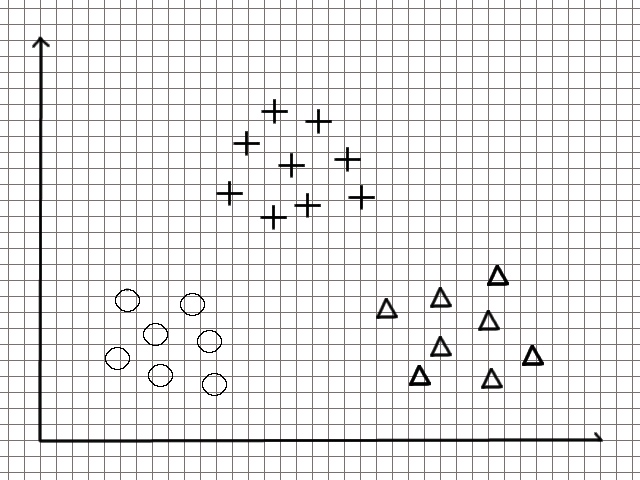
\includegraphics[width=0.75\linewidth]{multiclass_original} 
    \caption{Classes originais} 
    \vspace{4ex}
  \end{subfigure}%% 
  \begin{subfigure}[b]{0.5\linewidth}
    \centering
    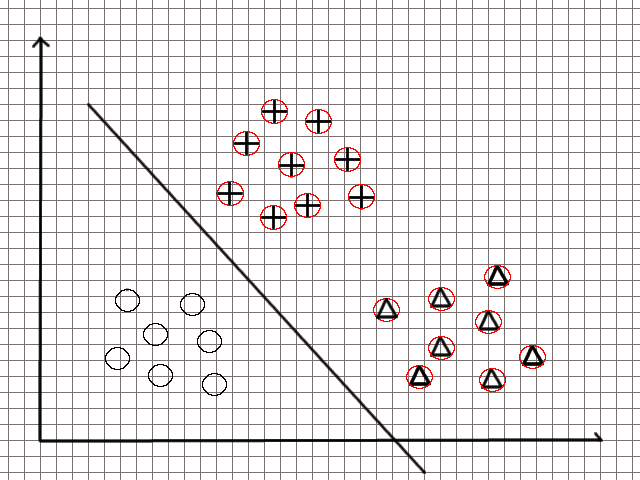
\includegraphics[width=0.75\linewidth]{multiclass_ova1} 
    \caption{Classificador para a classe 1} 
    \vspace{4ex}
  \end{subfigure} 
  \begin{subfigure}[b]{0.5\linewidth}
    \centering
    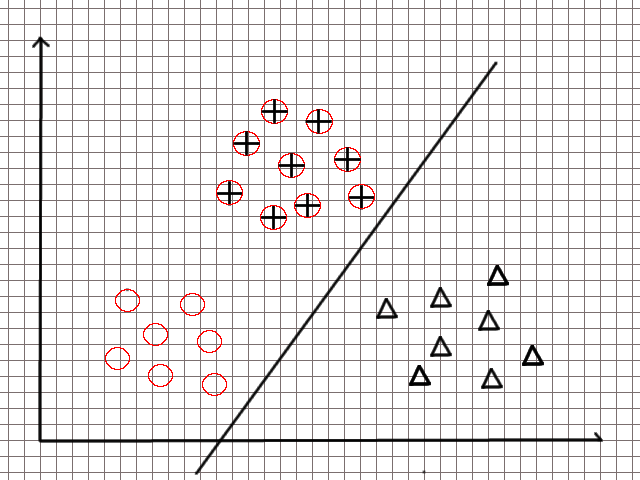
\includegraphics[width=0.75\linewidth]{multiclass_ova2} 
    \caption{Classificador para a classe 2} 
  \end{subfigure}%%
  \begin{subfigure}[b]{0.5\linewidth}
    \centering
    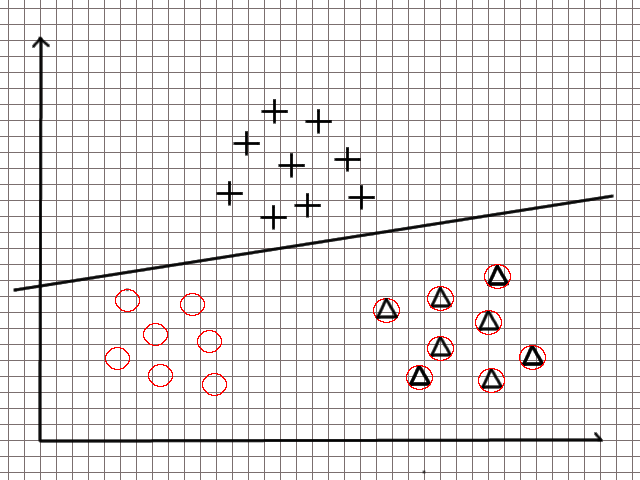
\includegraphics[width=0.75\linewidth]{multiclass_ova3} 
    \caption{Classificador para a classe 3} 
  \end{subfigure} 

\end{figure}

\section{Análise de Sentimentos}

O campo de análise de sentimentos, também conhecido como mineração de opinião é uma área da
ciência da computação que analisa as opiniões, sentimentos e atitudes das pessoas em relação
a uma entidade (Bing Liu, 2012)\citep{bingliu2012}. Uma entidade pode ser definida como o sujeito ao qual está
se observando as opiniões, seja ela uma pessoa, instituição ou produto.

A área possui uma diversa gama de aplicações, dentre elas, a área de classificação de sentimentos
que através do uso de informações subjetivas contidas num texto avalia qual a opinião relacionada
ao mesmo.

Classificação de sentimentos teve um crescimento devido à expansão da Web 2.0 que fez com que
as pessoas manifestassem suas opiniões e sentimentos através de blogs, fóruns, redes sociais
e páginas de reviews de produtos que, consequentemente fez com que empresas e pessoas de interesse
tivessem um acesso mais aberto e fácil a essas opiniões. O fácil acesso às opiniões dos usuários
junto com o grande volume delas tornou a análise manual um processo muito custoso, tornando
necessário recorrer a métodos automatizados para a análise e sumarização desses dados que
acabou por fim impulsionando estudos na área (Petković e Ringsquandl, 2013)\citep{petkovic2013}.

Bing Liu (2012)\cite{bingliu2012} divide as formas de classificar sentimentos 
em um documento em quatro formas:
\begin{itemize}
	\item Entidade:  um produto, pessoa sobre o qual o texto se refere, seja direta ou indiretamente.
	Nessa tarefa procura-se analisar se a opinião do texto em torno de uma entidade é positiva ou
	não.
	\item Aspecto: características sobre uma entidade. Por exemplo, se tem-se uma entidade que é um
	produto, aspectos de um produto poderiam ser material ou preço. Nessa forma procura-se avaliar
	a opinião acerca de cada um dos aspectos.
	\item Sentença: esse tipo de análise trabalha com o sentimento associado a cada sentença de
	um documento.
	\item Documento: nesse caso analisa-se o sentimento associado a um documento como um todo, 
	tratando de uma forma mais genérica em relação aos demais.
\end{itemize}

Comum a todas as formas de se analisar as opiniões de um documento é o uso dos métodos
para obter a opinião. Há duas abordagens para esse problema de classificação: a de aprendizado
de máquina (que iremos utilizar nesse trabalho) que consiste no uso de algoritmos de 
classificação em conjunto com técnicas de processamento de texto (que será explicado nas próximas
seções) e a abordagem com um dicionário léxico onde a análise é feita baseada na pontuação
entre palavras positivas e negativas contidas no documento (Medhat et al., 2014) \citep{medhat2014}.

No caso desse trabalho, foi escolhido a análise em torno do documento / sentença (devido à estrutura
dos tuítes tem-se que os documentos são, em sua maioria, compostos por apenas uma 
sentença). 

\subsection{Análise de tuítes de política}

Dentre os domínios de aplicação da classificação de sentimentos, escolheu-se como domínio o
escopo político. Nesse caso, tem-se que as entidades nos documentos são constituídas por
políticos e projetos de lei. E neste trabalho serão analisados tuítes.

O Twitter desde as eleições presidenciais estadunidenses de 2008 mostrou influência
na decisão das eleições evidenciado pela campanha online realizada pela equipe do
candidato Barack Obama (Petković e Ringsquandl, 2013)\citep{petkovic2013}. Desde então, 
a rede social tem sido usada não só para a campanha de políticos, mas também para a avaliação
da opinião em relação às medidas tomadas por eles. 
A escolha foi feita tendo em vista o uso da rede social 
para expressar opiniões sobre diversos assuntos, incluindo política.


\subsection{Obtendo um vetor de \textit{features}}
\label{subsec:featurization}

Para realizar a extração das informações do texto, existe uma etapa de pré-processamento na qual
cada texto é transformado num vetor numérico para então ser processado por algum algoritmo de
classificação, as mais famosas são o modelo \textit{bag of words} (BOW) e o n-grama. 


Antes de obter um vetor de \textit{features}, é feito um pré-processamento no documento removendo 
\textit{stop-words} (palavras muito usadas na língua portuguesa como artigos e preposições), caracteres 
especiais, adicionando espaços antes e depois  de pontuações e transformando
em um vetor de \textit{tokens} com cada token representando as palavras do texto. 
Uma vez que foi obtido o vetor de \textit{tokens}, é removido todo 
elemento que seja apenas espaço e pontuação.

Na abordagem n-grama os termos não são apenas as palavras, mas
um conjunto de $n$ palavras juntas, o que traz mais informação pelo fato de juntar substantivo e verbo, substantivo e adjetivo, por exemplo, entretanto acaba gerando um vetor de \textit{features}
ainda maior que, consequentemente, faz com que os algoritmos demorem mais para convergir \cite{ngram}. A figura 
\ref{fig:ngram} exemplifica o funcionamento do n-grama.


\begin{figure}[H]
	\centering	
	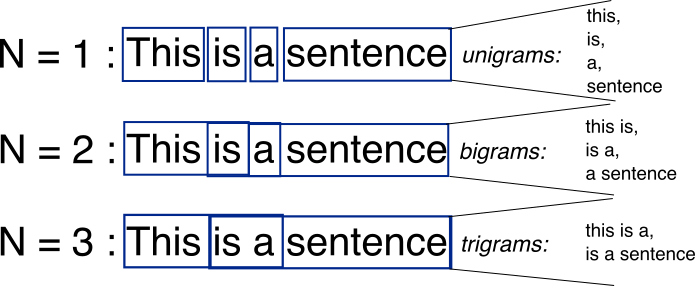
\includegraphics[scale=0.5]{n_gram}
	\caption{Funcionamento do n-grama para $n = 1, 2$ e $3$}
	\label{fig:ngram}
\end{figure}

Na abordagem usando o BOW, constrói-se uma matriz de entrada onde cada linha i representa um documento 
(texto sobre o qual quer extrair a opinião) e as colunas representam a frequência de um termo, o 
conjunto de todos os textos é chamado de \textit{corpus} \cite{bow}. O funcionamento do BOW é ilustrado em \ref{fig:bow}.

\begin{figure}[H]
	\centering
	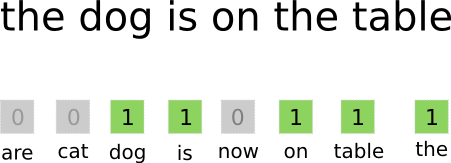
\includegraphics[scale=0.5]{bow}
	\caption{Funcionamento do \textit{Bag-of-Words}}
	\label{fig:bow}
\end{figure}

A escolha pelo BOW foi tida baseada no compromisso entre desempenho e performance do algoritmo.

Após tokenizar os textos, monta-se uma nova \textit{string} juntando todas as \textit{tokens} usando espaços para então montar um vetor de frequência a partir do novo \textit{corpus} higienizado.

A medida de frequência de um termo 
pode ser uma medida simples como a quantidade de vezes em que um termo j aparece no documento
i ou se o termo j aparece no documento i (nesse caso cada vetor de entrada seria um vetor binário) bem
como pode ser uma medida mais complexa como tf-idf (\textit{term frequency - inverse document frequency}).
A relação entre os métodos de computar a frequência e o desempenho dos algoritmos de classificação serão
exibidas no capítulo seguinte.

O método tf-idf baseia-se na frequência de cada termo ponderada pela frequência inversa no documento,
que é usada para mensurar o quão importante um termo é em um documento (por exemplo a palavra "um" em
um conjunto de textos em português aparece várias vezes, apesar de ter uma baixa importância) \cite{tf-idf}. 
Ele pode ser calculado pelas expressões:

\begin{center}
	\begin{dgroup}
		\begin{dmath}
			TF(t) = \frac{\text{\# de aparições de t no documento}}{\text{total de termos no documento}} 
		\end{dmath}
		\begin{dmath}
			IDF(t) = log \left(  \frac{\text{Total de documentos}}{\text{\# de documentos que contenham t}} \right) 
		\end{dmath}	    
		\begin{dmath}
			TF-IDF(t) = TF(t)*IDF(t)
		\end{dmath} 	    
	\end{dgroup}
\end{center}

Abaixo será dado um exemplo de como funciona o processo de vetorização por frequências e por
tf-idf.

O corpus em questão é constituído pelos seguintes textos:

\begin{enumerate}
	\item Eu amo cachorros
	\item Eu odeio cachorros e costurar
	\item Costurar é meu hobby e meu amor
\end{enumerate}

Construindo o vocabulário e realizando a vetorização, obtém-se os vetores de frequência descritos na tabela abaixo, o
cabeçalho da tabela representa o vocabulário.

\begin{tabular}{| c | c | c | c | c | c | c | c | c | c | c | c |}
\hline
& eu & amo & cachorros & odeio & e & costurar & é & meu & hobby & amor \\ \hline
Vetor 1 & 1 & 1 & 1 & 0 & 0 & 0 & 0 & 0 & 0  & 0  \\ \hline
Vetor 2 & 1 & 0 & 1 & 1 & 1 & 1 & 0 & 0 & 0 & 0  \\ \hline
Vetor 3 & 0 & 0 & 0 & 0 & 1 & 1 & 1 & 2 & 1 & 1  \\ \hline
\end{tabular}

Já usando calculando o valor tf-idf para cada um, obtém-se os seguintes vetores:

\begin{tabular}{| c | c | c | c | c | c | c | c | c | c | c | c |}
\hline
& eu & amo & cachorros & odeio & e & costurar & é & meu & hobby & amor \\ \hline
Vetor 1 & 0.18 & 0.48 & 0.18 & 0 & 0 & 0 & 0 & 0 & 0  & 0  \\ \hline
Vetor 2 & 0.18 & 0 & 0.18 & 0.48 & 0.18 & 0.18 & 0 & 0 & 0 & 0  \\ \hline
Vetor 3 & 0 & 0 & 0 & 0 & 0.18 & 0.18 & 0.48 & 0.95 & 0.48 & 0.48  \\ \hline
\end{tabular}


O procedimento da obtenção do vocabulário utilizando o BOW e vetorização dos textos, independente da
medida de frequência, foi feito utilizando o módulo \texttt{feature_extraction} da biblioteca
\texttt{scikit-learn}. Um exemplo de código onde é realizado todo o processo de vetorização descrito
nesta subseção pode ser encontrado em \url{https://github.com/romaolucas/bow}.

\subsection{Classificação manual da opinião}

Com o conjunto de dados obtido em \ref{subsec:featurization}, podemos aplicar os algoritmos 
descritos no começo do capítulo. Entretanto como também mencionado no começo deste capítulo,
problemas de aprendizado supervisionado exigem que o conjunto de dados seja composto não só dos
dados, mas também do valor esperado para cada entrada. No caso da classificação da opinião de
textos, tal opinião deve ser primeiro atribuída manualmente para que, com posse dessas opiniões,
seja possível treinar os algoritmos.

Para facilitar a etapa de classificação manual, foi desenvolvido um sistema online onde cada usuário
informa a quantidade de tuítes que deseja classificar e consegue classificá-los de forma
mais simples. Deu-se a essa ferramenta o nome de CLAM (de Classificador Manual).

O desenvolvimento do CLAM foi motivado pela ausência de ferramentas no Brasil que permitem a
colaboração nessa etapa de classificação manual (uma ferramenta comumente usada é o \textit{Amazon
Mechanical Turk}, porém na época do desenvolvimento do CLAM não estava disponível no Brasil)
em conjunto com a falta de ferramentas gratuitas de 
uma forma geral, uma vez que a maioria das ferramentas existentes são pagas (vide o 
próprio \textit{Amazon Mechanical Turk}). Por isso priorizou-se construir um código simples
para que fosse fácil a modificação da base do sistema por colaboradores externos,
que fosse de fácil uso para o usuário final e também de fácil hospedagem do sistema
em alguma plataforma como Heroku e Firebase.

O código é de domínio público e está disponível no link:
 \url{https://github.com/romaolucas/manual-classifier-helper}

O projeto foi desenvolvido usando a linguagem Python em conjunto do \textit{framework} web
Django por já possuir diversas ferramentas integradas não só de gerenciamento do sistema, bem como
modelagem do banco de dados e sistema de migração para que possa modificar os modelos de dados já
existentes sem precisar realizar um acesso direto à base de dados além de possuir um conjunto
de bibliotecas que facilitam o processo de importação de dados em csv e vasta quantidade de 
tutoriais de como desenvolver uma aplicação usando Django.

Para a modelagem de dados construiu-se dois modelos: um para tuítes e outro para
as opiniões.
Na modelagem, considerou-se que cada usuário irá classificar apenas textos que não 
possuem uma classificação, não só para evitar ter que lidar com opiniões divergentes em um texto,
mas também para garantir um maior número de dados para o treinamento. 

O CLAM possui o seguinte fluxo para a classificação:

\begin{enumerate}
	\item Informa a quantidade de tuítes que se deseja classificar.
	\begin{figure}[H]
		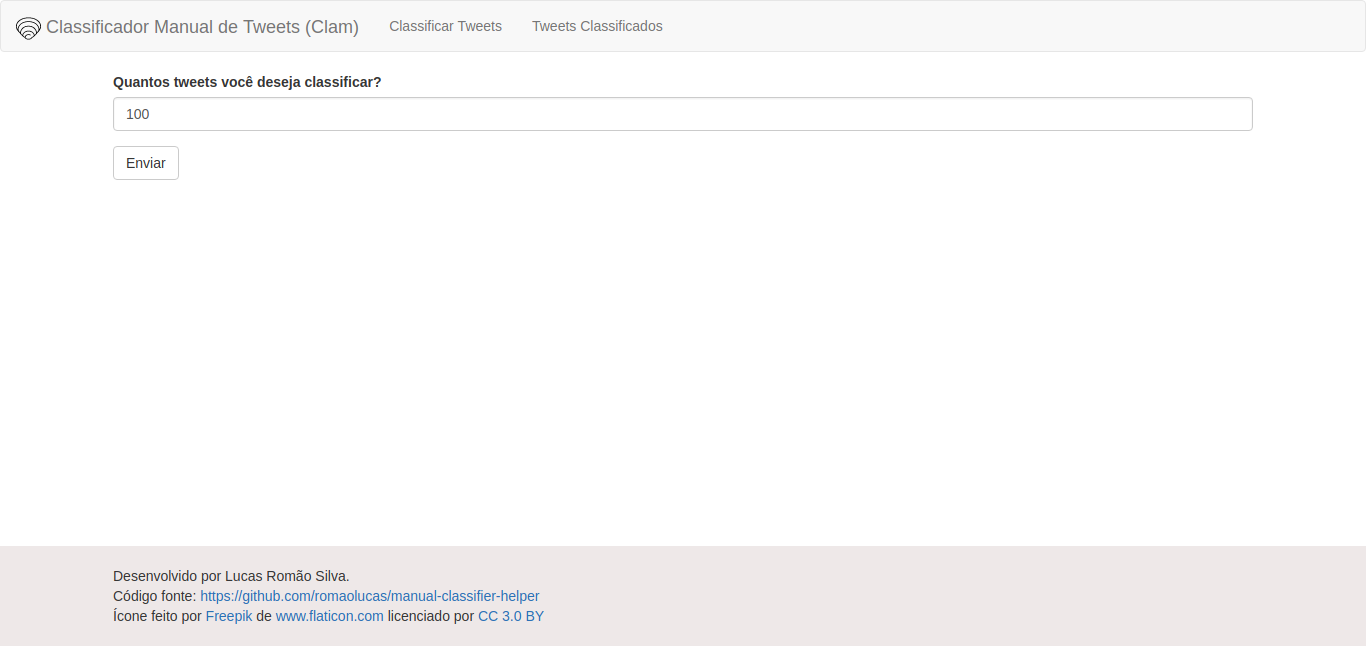
\includegraphics[scale=0.27]{clam_inicio}
	\end{figure}
	\item O usuário é levado a uma página com os n tuítes para classificar.
	Enquanto o campo da opinião é obrigatório, existe um campo optativo para informar
	se o tuíte é irônico ou não, uma vez que textos com ironia atrapalham
	o treinamento por conter palavras positivas sendo usadas de maneira negativa e vice-versa.
	\begin{figure}[H]
		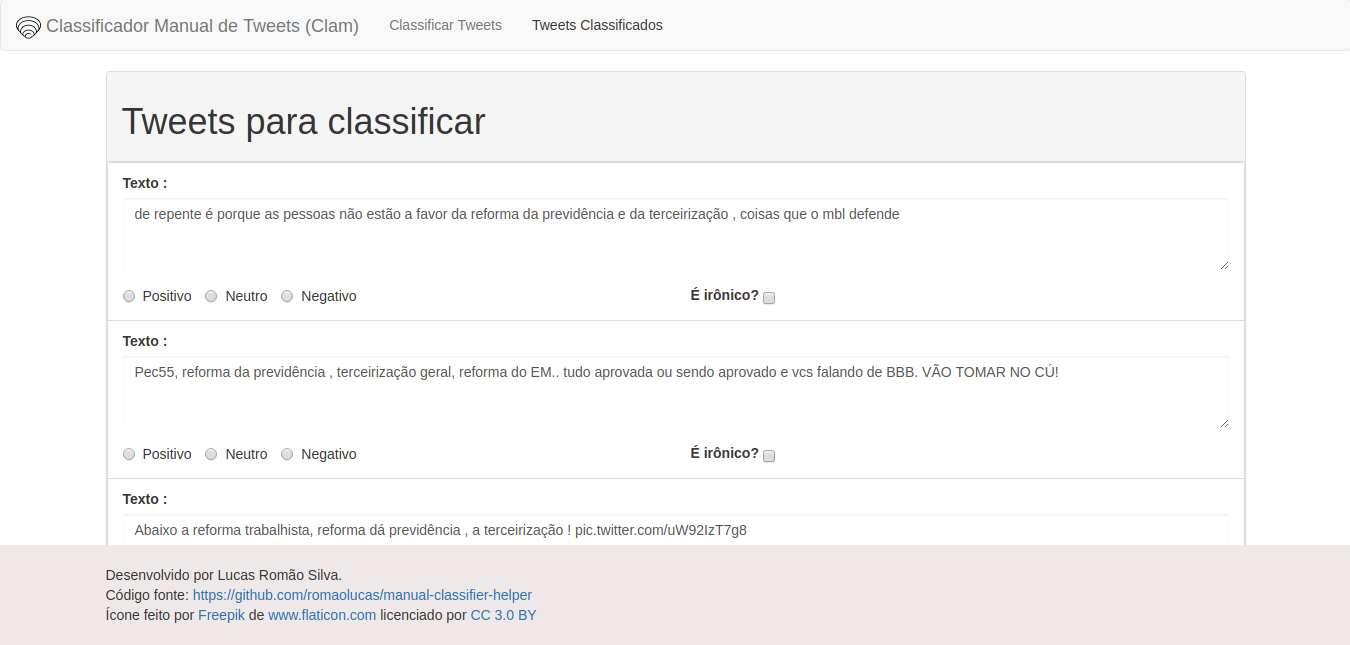
\includegraphics[scale=0.27]{clam_classificar}
	\end{figure}
	\item Uma vez classificados, o usuário é levado a uma página onde é possível ver todos
	os tuítes já classificados e também gerar um arquivo csv contendo todos aqueles
	que não foram marcados como irônicos.
	\begin{figure}[H]
		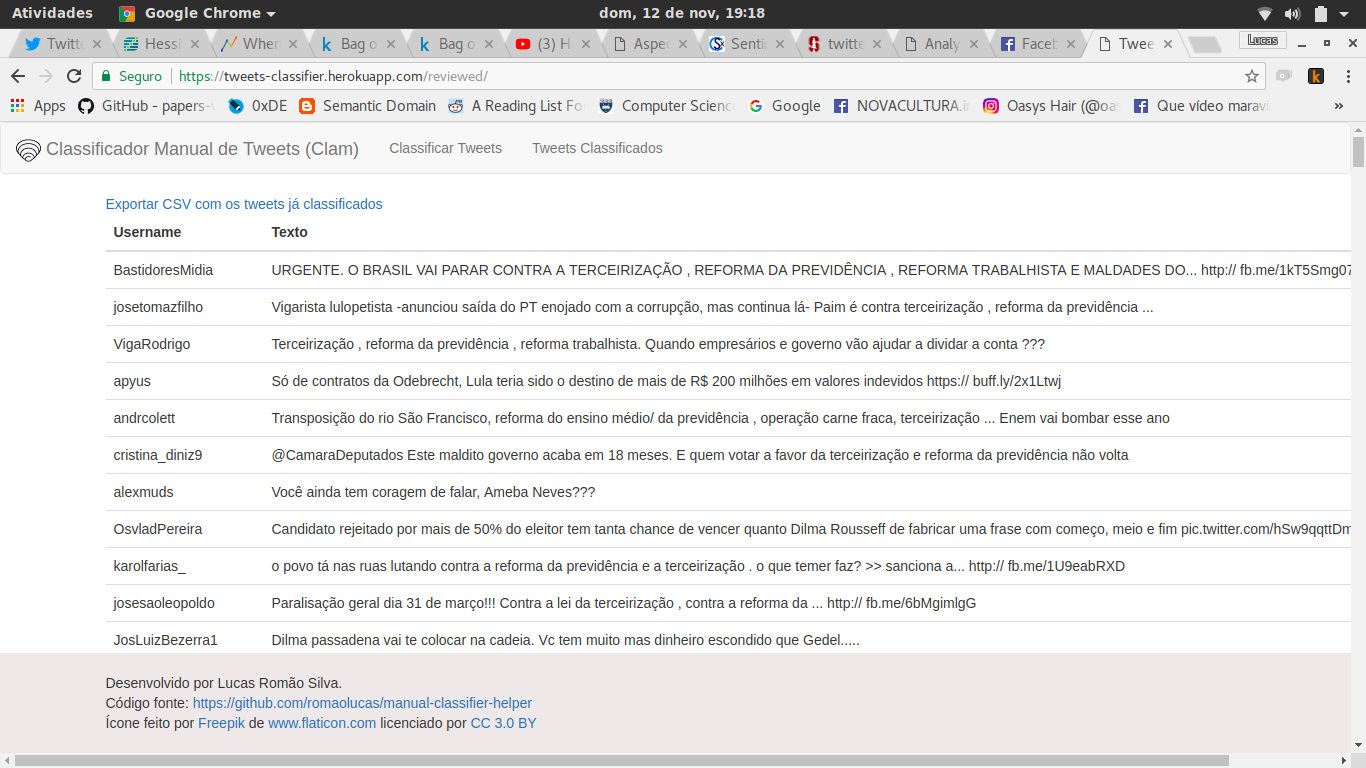
\includegraphics[scale=0.27]{clam_classificados}
	\end{figure}
\end{enumerate}

Para um usuário que deseja hospedar a plataforma e usá-la para si, existe também o admin onde
é possível importar tuítes para serem classificados.

Abaixo é descrito o fluxo para a importação de novos dados no admin.

\begin{enumerate}
	\item Realiza o login no sistema utilizando seu usuário e senha de administrador.
	\begin{figure}[H]
		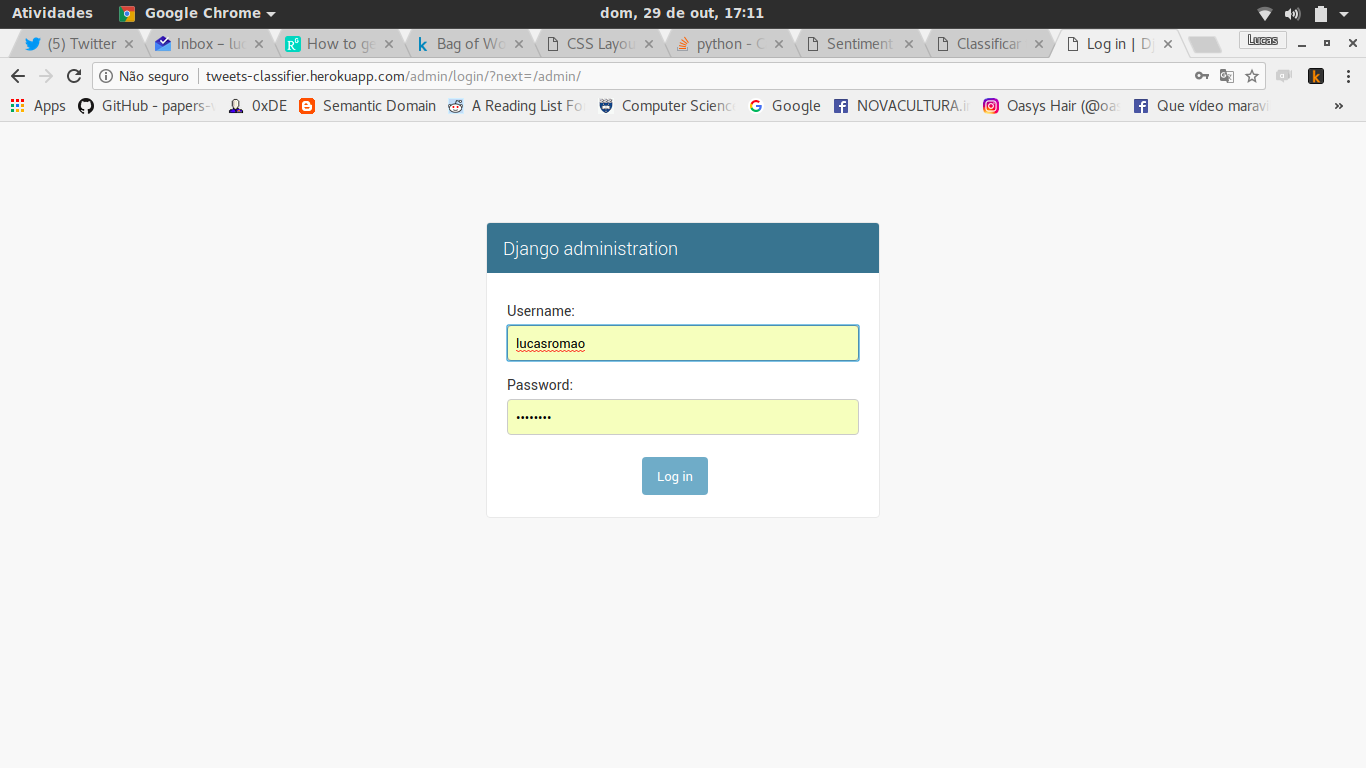
\includegraphics[scale=0.27]{clam_login}
	\end{figure}
	\item Seleciona a parte de Tweets na tela principal.
	\begin{figure}[H]
		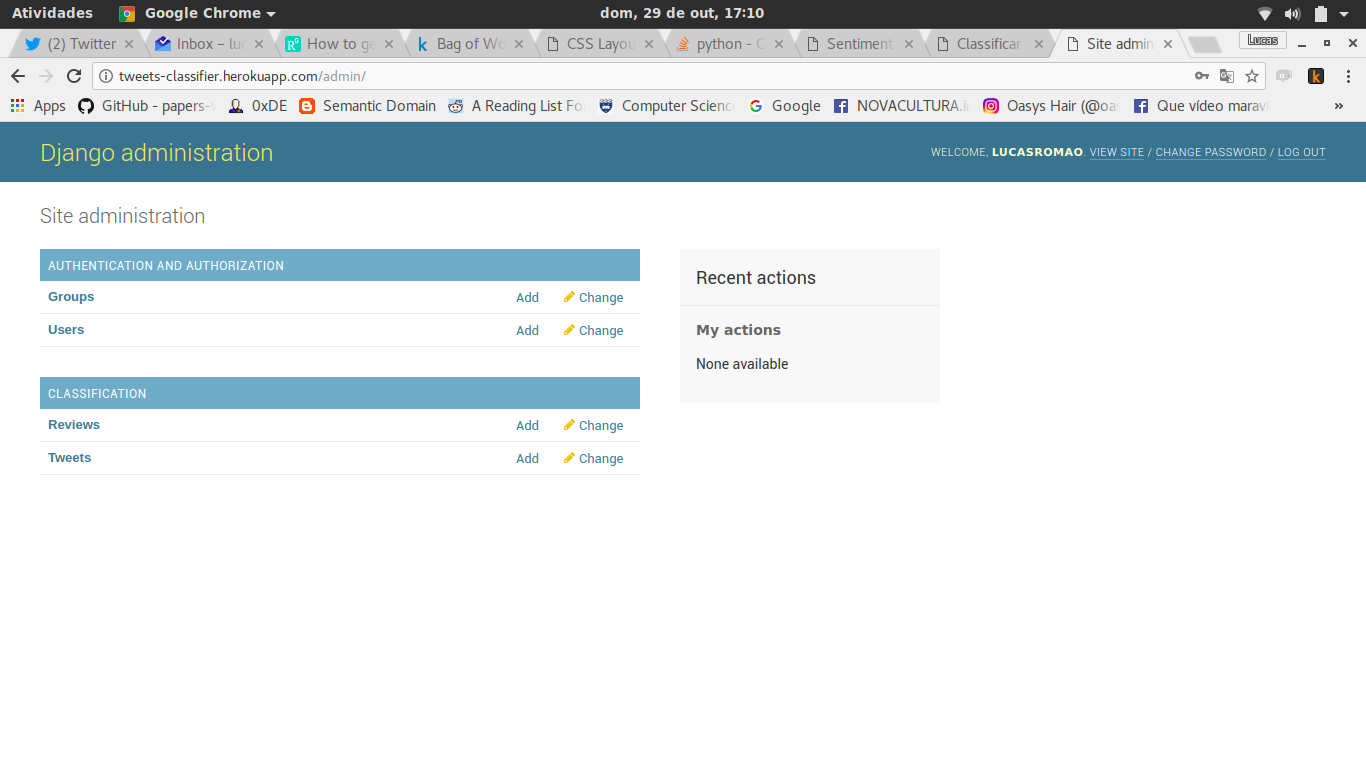
\includegraphics[scale=0.27]{clam_admin}
	\end{figure}
	\item Uma vez na parte de visualizar todos os tuítes já armazenados na base de dados,
	seleciona a opção de importar no canto superior direito.
	\begin{figure}[H]
		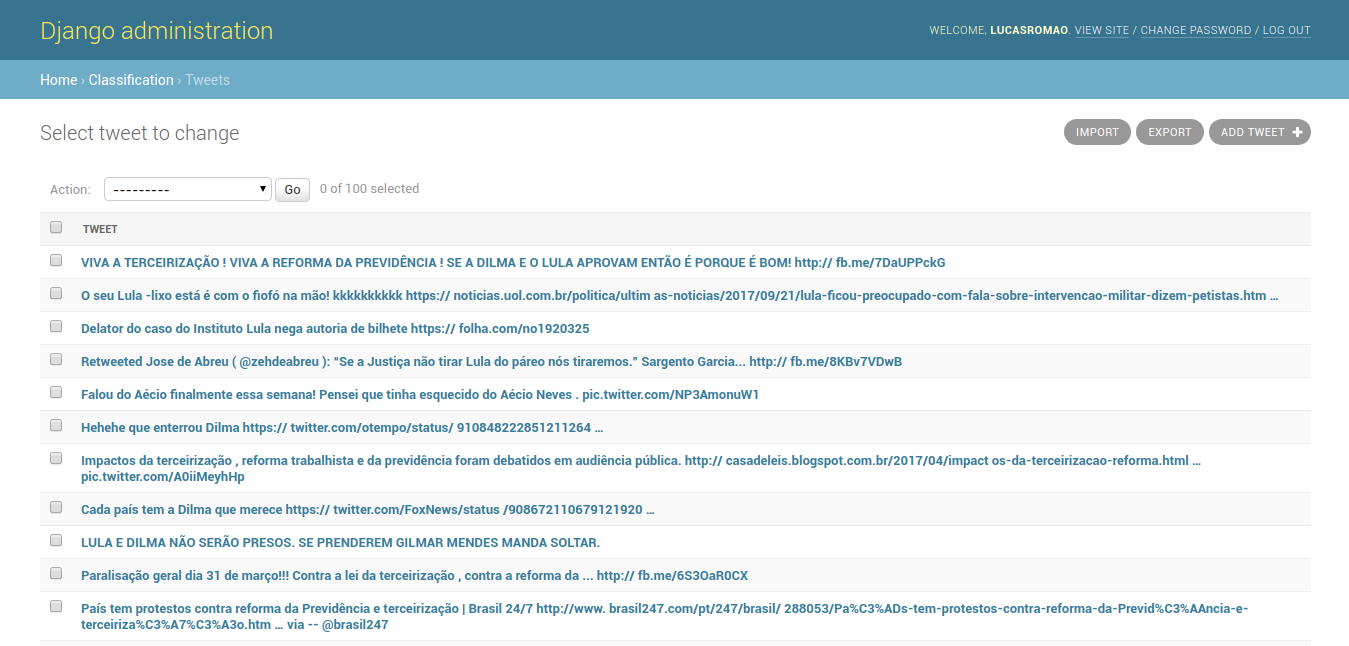
\includegraphics[scale=0.27]{clam_tweets}
	\end{figure}
	\item Na página que segue, basta informar um arquivo .csv, .xls (formato do excel) ou .json
	contendo nessa ordem: o id do tuíte (fornecido pelo Twitter), usuário que escreveu, 
	texto, espaço vazio para representar o id que será preenchido automaticamente na hora de 
	importar no banco de dados.
	\begin{figure}[H]
		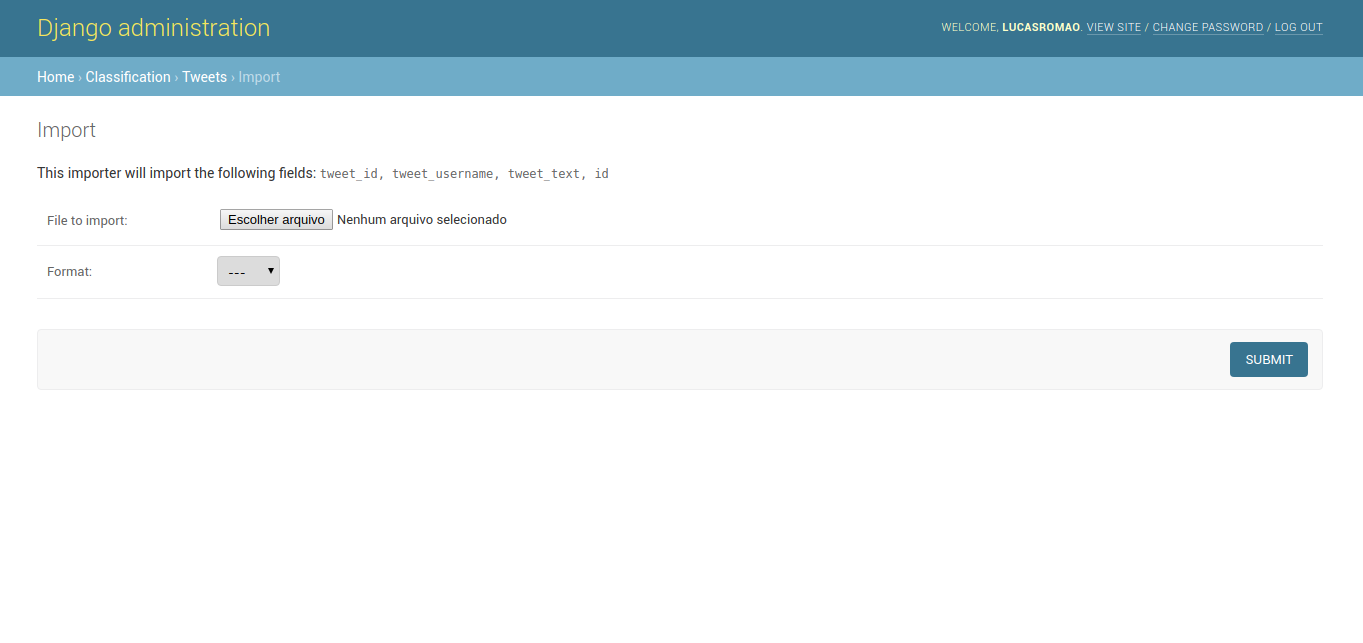
\includegraphics[scale=0.2]{clam_importador}
	\end{figure}
	\item Caso todos os dados sejam fornecidos corretamente, será passado a uma nova página para
	confirmar se deseja importar e, por fim, será redirecionado à pagina que contém todos os
	tuítes.
\end{enumerate}

No apêndice \ref{chap:clam} é descrito em detalhes como instalar e realizar as
configurações iniciais do CLAM.
